\section{Motivations}
\begin{figure*}[t]
    \centering
    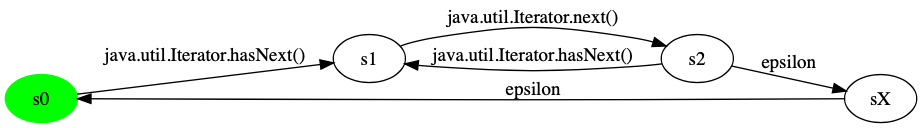
\includegraphics[width=0.77\textwidth]{figures/motivation/sample.png}
    \caption{Sample of the generated transition system for \texttt{java.util.Iterator}}
    \label{fig:motivation}
\end{figure*}
\pouria{I have added all of the hypothesis that we have about the reasons that model-seeding can perform better than other strategies to this section. However, I am not sure if this is the best place for this discussion. At this point in the paper, readers are not that much family about the previous studies. So, maybe this discussion confuses them here. Perhaps, adding it at the end of the background is more logical. we can change the name of the background section to background and motivations.}
The existing seeding techniques use only one resource to collect information for seeding. However, it is possible that the preferred resource does not have enough information about the usages of the interesting classes. For instance, test seeding only uses the carved call sequences from the execution of the existing test cases. If the existing test cases do not cover the behavior of the crash in the interesting classes, this seeding strategy may even misguide the search process. On the contrary, the behavioral model seeding collects the call sequences of each class from various resources and use all of them to infer a centralized transition system which represents the class usage. Since this strategy uses more resources compared to the other seeding strategies, it has a higher chance to seed a sequence which is closer to the crash reproducing scenario.

The improvement that we can achive Behavioral model seeding merges the observed call sequences to infer a transition system. This merging process may produce different sequences from the existing ones. For instance, Figure \ref{fig:motivation} demonstrates the generated transition system for java class \texttt{java.util.Iterator} from two call sequences: (\texttt{hasNext()}, \texttt{next()}) and (\texttt{hasNext()}, \texttt{next()},\texttt{hasNext()}, \texttt{next()}). This transition system contains a loop. So, the generated test from this mode can contain more than 2 method calls to the \texttt{next()} method.


If the number of observed call sequences is large, the seeding strategy needs a procedure to prioritize the call sequences for seeding. Seeding the random call sequences can misguide the search process. The existing seeding strategies do not have any procedure to fulfill this requirement. Behavioral model seeding uses the generated transition systems to define a technique for prioritizing the seeding candidates.
